\documentclass{ximera}
\input{preamble}
\input{orccaImagePreamble}
\usepackage{hyperref}
\usepackage{lipsum}
\usepackage{lmodern}
\usepackage{tcolorbox}



\author{Elizabeth Miller}
%\license{Creative Commons 4.0 International License}



\title{Relations and Graphs: Famous Functions}

\begin{document}

\begin{abstract}
We list important relations and functions that will be explored throughout this course and used often in Calculus.
\end{abstract}
\maketitle

%\typeout{************************************************}
%\typeout{Famous Functions and Relations}
%\typeout{************************************************}

\section{Famous Functions and Relations} 
Throughout this course and in Calculus you will study certain relations in depth.  These relations are usually functions, and they are the functions that come up often in real world applications.  In this section, we will give you a list of some of these functions, including their algebraic equation, their graph, and a table of some of their most important values.  You may never have seen some of these functions before and you might not know what their algebraic expressions mean.  That is ok.  We will learn more about them throughout this course.  Remember, though, that a relation or function can be given by a graph.  For now, familiarize yourself with these graphs.  They will come up in examples throughout the course.

%\typeout{************************************************}
%\typeout{Lines}
%\typeout{************************************************}

\subsection{Lines}
Of the most important types of functions is a line.  

\begin{example}
$y=x$ is a line.

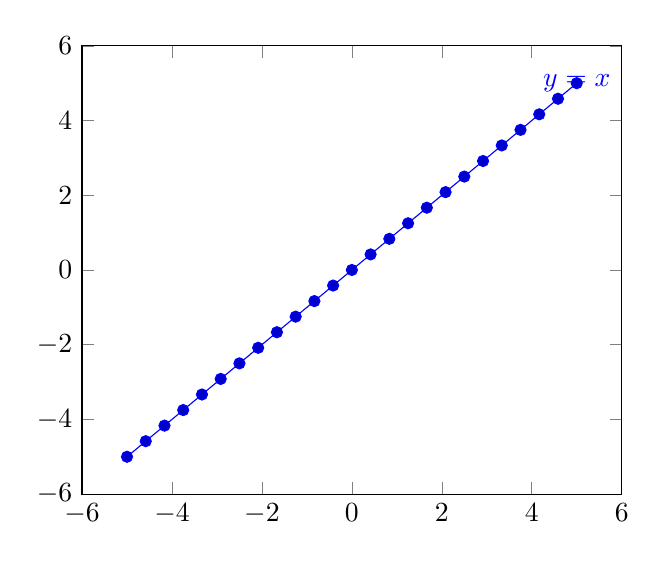
\begin{tikzpicture}
    \begin{axis}
        \addplot{x} node{$y=x$};
    \end{axis}
\end{tikzpicture}

\begin{tabular}{ |c || c|  }
 \hline
 \multicolumn{2}{|c|}{Important Values of $y=x$} \\
\hline
 \hline
 x & y\\
 \hline
 0&0\\
 1&1\\
 2&2\\
 -1&-1\\
 -2&-2\\
 \hline
\end{tabular}

\end{example}

In general, lines can be written as $y=mx+b$ where $m$ and $b$ can be any numbers.  You can play with changing the values of $m$ and $b$ on the graph using Desmos and see how that changes the graph of the line.  

\begin{center}  
\desmos{japnhapzvn}{800}{600}  
\end{center}


%\typeout{************************************************}
%\typeout{Parabolas}
%\typeout{************************************************}

\section{Parabolas}
Another important type of function is a parabola.  

\begin{example}
$y=x^2$ is a parabola.

\begin{tikzpicture}
    \begin{axis}
        \addplot[smooth]{x^2} node{$y=x^2$};
    \end{axis}
\end{tikzpicture}

\begin{tabular}{ |c || c|  }
 \hline
 \multicolumn{2}{|c|}{Important Values of $y=x$} \\
\hline
 \hline
 x & y\\
 \hline
 0&0\\
 1&1\\
 2&4\\
 -1&1\\
 -2&4\\
 \hline
\end{tabular}

\end{example}

In general, parabolas can be written as $y=ax^2+bx+c$ where $a$, $b$, and $c$ can be any numbers.  You can play with changing the values of $a$, $b$, and $c$ on the graph using Desmos and see how that changes the graph of the parabola.  

\begin{center}  
\desmos{nmlghfrws9}{800}{600}  
\end{center}



%\typeout{************************************************}
%\typeout{Absolute Value}
%\typeout{************************************************}

\section{Parabolas}
Another important type of function is the absolute value function.  This is the function that takes all y-values and makes them positive.  

\begin{example}
$y=x^2$ is a parabola.

\begin{tikzpicture}
    \begin{axis}
        \addplot[smooth]{x^2} node{$y=x^2$};
    \end{axis}
\end{tikzpicture}

\begin{tabular}{ |c || c|  }
 \hline
 \multicolumn{2}{|c|}{Important Values of $y=x$} \\
\hline
 \hline
 x & y\\
 \hline
 0&0\\
 1&1\\
 2&4\\
 -1&1\\
 -2&4\\
 \hline
\end{tabular}

\end{example}

In general, parabolas can be written as $y=ax^2+bx+c$ where $a$, $b$, and $c$ can be any numbers.  You can play with changing the values of $a$, $b$, and $c$ on the graph using Desmos and see how that changes the graph of the parabola.  

\begin{center}  
\desmos{nmlghfrws9}{800}{600}  
\end{center}



%\typeout{************************************************}
%\typeout{Square Root}
%\typeout{************************************************}

\section{Square Root}
Another famous function is the square root function, $y=\sqrt{x}$.


\begin{tikzpicture}
    \begin{axis}
        \addplot[samples=200,domain=0:30]{sqrt(x)};
    \end{axis}
\end{tikzpicture}

\begin{tabular}{ |c || c|  }
 \hline
 \multicolumn{2}{|c|}{Important Values of $y=\sqrt{x}$} \\
\hline
 \hline
 x & y\\
 \hline
 0&0\\
 1&1\\
 4&2\\
 9&3\\
 25&5\\
 \hline
\end{tabular}


%\typeout{************************************************}
%\typeout{Exponential}
%\typeout{************************************************}

\section{Exponential}
Another famous function is the exponential growth function, $y=e^x$.  Here $e$ is the mathematical constant known as Euler's number.  It is approximately 2.71828.

\begin{tikzpicture}
    \begin{axis}
        \addplot[samples=200,domain=-10:4]{e^x};
    \end{axis}
\end{tikzpicture}

\begin{tabular}{ |c || c|  }
 \hline
 \multicolumn{2}{|c|}{Important Values of $y=e^x$} \\
\hline
 \hline
 x & y\\
 \hline
 0&1\\
 1&e\\
 -1&$\frac{1}{e}$\\
 \hline
\end{tabular}

In general, we can talk about exponential functions of the form $y=a^{bx}$ where $a$ is a positive number and $b$ is any number.  You can play with changing the values of $a$ and $b$ on the graph using Desmos and see how that changes the graph.  

\begin{center}  
\desmos{lylujzszb1}{800}{600}  
\end{center}



%\typeout{************************************************}
%\typeout{Logarithms}
%\typeout{************************************************}

\section{Logarithm}
Another group of famous functions are logarithms.

\begin{example}
$y=\ln(x)=\log_e(x)$.  Here $e$ is the mathematical constant known as Euler's number.  It is approximately 2.71828.

\begin{tikzpicture}
    \begin{axis}
        \addplot[samples=200,domain=0.01:8]{ln(x)};
    \end{axis}
\end{tikzpicture}

\begin{tabular}{ |c || c|  }
 \hline
 \multicolumn{2}{|c|}{Important Values of $y=ln(x)$} \\
\hline
 \hline
 x & y\\
 \hline
 1&0\\
 e&1\\
 $\frac{1}{e}$&-1\\
 \hline
\end{tabular}

You may notice that the table of values for $y=ln(x)$ and $y=e^x$ are similiar.  This is becase these two functions are interconnected to one another.  We will explore this more later in the course.

\end{example}

In general, we can talk about exponential functions of the form $y=log_b(x)$ where $b$ is a positive number.  You can play with changing the values of $b$ on the graph using Desmos and see how that changes the graph.  

\begin{center}  
\desmos{lxllnpdi6w}{800}{600}  
\end{center}

%\typeout{************************************************}
%\typeout{Sine}
%\typeout{************************************************}

\section{Sine}
Another important function is the sine function, $y=sin(x)$. 

\begin{example}
$y=(x)=\sin(x)$.  This function comes from trigonometry. In the table below we will use another mathematical constant, $\pi$ ("pi" pronounced pie) which is approximately 3.14159.

\begin{tikzpicture}
    \begin{axis}[ymin=-2, ymax=2,
		   %xtick={-6.28318, -4.7123889, -3.14159, -1.5708, 1.5708, 3.14159, 4.7123889, 6.28318},
    xticklabels={
        $-2\pi$, $-\frac{3\pi}{2}$, $-\pi$, $\frac{\pi}{2}$,
        $\frac{\pi}{2}$, $\pi$, $\frac{3\pi}{2}$, $2\pi$
    }, ]
        \addplot[samples=200]{sin(deg(x))};
    \end{axis}
\end{tikzpicture}

\begin{tabular}{ |c || c|  }
 \hline
 \multicolumn{2}{|c|}{Important Values of $y=sin(x)$} \\
\hline
 \hline
 x & y\\
 \hline
 \hline
 $-\pi$&0\\
 \hline
 $\frac{-\pi}{2}$&-1\\
 \hline
 0&0\\
 \hline
 $\frac{\pi}{2}$&1\\
 \hline
 $\pi$&0\\
 \hline
$\frac{3\pi}{2}$&-1\\
 \hline
 $2 \pi$&0\\
 \hline
\end{tabular}

\end{example}

In general, we can consider $y=asin(bx)$.  You can play with changing the values of $a$ and $b$ on the graph using Desmos and see how that changes the graph.  

\begin{center}  
\desmos{vkxzcfv2aq}{800}{600}  
\end{center}

\end{document}
